% !TeX encoding = windows-1251
\documentclass[a4paper,12pt]{article}
\usepackage{newlistok}
\usepackage{tikz}

\УвеличитьВысоту{1.5cm}
\УвеличитьШирину{1.5cm}
\renewcommand{\spacer}{\vspace{1mm}}

\Заголовок{Самостоятельная работа}
\def\словоЛисток{СР \No\/}
\НомерЛистка{2}
\ДатаЛистка{5 ноября 2012г.}

\begin{document}


\ncopy{3}{
%\vspace*{-12mm}
\СоздатьЗаголовок

\задача
\пункт 
Докажите, что $n\cdot C_{n-1}^{k-1} = k\cdot  C_n^k$.
\пункт
Докажите это тождество комбинаторными методами, не используя явную формулу для $C_n^k$.
\кзадача

\задача
Сколько существует шестизначных чисел, у которых цифры идут в порядке возрастания?
\кзадача

\УстановитьГраницы{0cm}{3.5cm}
\задача
Докажите, что единица --- единственное число в треугольнике Паскаля, которое встречается в нём бесконечное количество раз.
\кзадача

\задача
Мизеров, Распасной и Шестирной играют в преферанс. 
Раздаются по 10 карт на руки и две в прикуп.
Какое количество раздач существует?
\кзадача

\сзадача
\putthere{160mm}{9mm}{%
      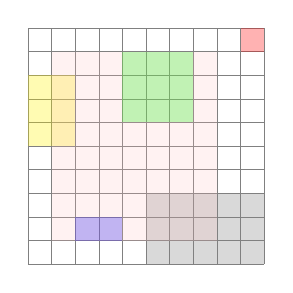
\begin{tikzpicture}
      [scale=.3
      ,fil/.style={color=green!50!white,opacity=.5}
      ,lin/.style={color=green!80!black,thick}
      ,lindot/.style={color=blue!50}
      ]
        \draw[step=1cm,gray,very thin] (0,0) grid (10cm,10cm);
        \fill[color=green, opacity= .3] (4,6) rectangle (7,9);
        \fill[color=blue, opacity= .3] (2,1) rectangle (4,2);
        \fill[color=yellow, opacity= .3] (0,5) rectangle (2,8);
        \fill[color=gray, opacity= .3] (5,0) rectangle (10,3);
        \fill[color=red, opacity= .3] (9,9) rectangle (10,10);
        \fill[color=pink, opacity= .2] (1,1) rectangle (8,9);
      \end{tikzpicture}
}{7cm}{}
Каким числом способов можно выбрать прямоугольник в квадрате $n\times n$?
\кзадача

\ВосстановитьГраницы


\hrl
\note{Для получения оценки $n$ необходимо правильно решить $n-1$ задачу. Решившие все 5 задач получают две пятёрки.\\
Можно пользовать любыми бумажными носителями информации. Задачи необходимо \выд качественно записать. }
}


%\ЛичныйКондуит{0mm}{6mm}
%\СделатьКондуит{6mm}{6mm}

\end{document}
